\section{Discussion}
We compared the correctness of the second users performances using using the Sorensen-Dice coefficient~\cite{sorensen1948method}. Figure~\ref{fig:Scatter} shows the offline users were more accurate than the real-time users. The offline users were more accurate in finding the movie recommendation in the last task. We observed an interesting pattern that for solving the task they devised a method. They started from the end of the task and went backward because generally the recommendation is answered at the end of the task in first study and it was likely that first users were looking at the movies they recommended at the end of that task. The real-time users got wrong in that case. They primarily chose the movie as soon as they identified the data as Recommendation task data. The offline users were more observant to the heatmap than the real-time users. The real-time users focused mainly on the labels which persisted for a while. The real-time users were less accurate in task time identification than the offline users. Generally in case of inaccurate task identification, the real-time users missed task transitions. 

\begin{figure}[htb]
  \centering
  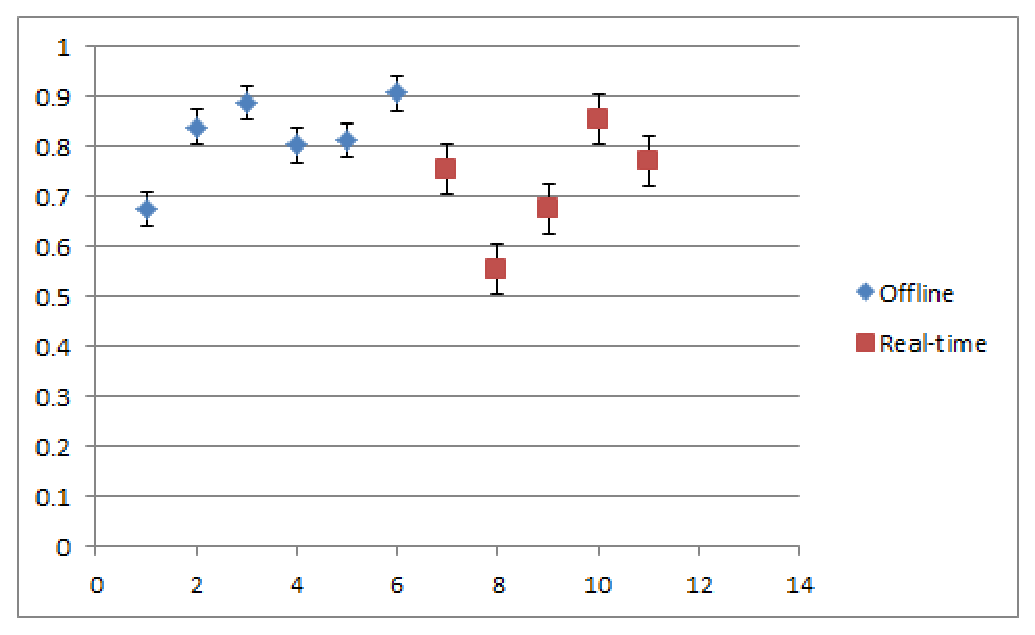
\includegraphics[width=\linewidth]{images/Scatter.eps}
  \caption{Correctness of users in the second study.}
	\label{fig:Scatter}
\end{figure} 
